W układzie przedstawionym na rysunku ciało \emph{A} o masie \emph{m} umieszczone zostało między dynamometrami \emph{B} i \emph{B'}. Wielkość ciała \emph{A} jest tak dobrana, że na nieważkie dynamometry w stanie spoczynku nie jest wywierane żadne działanie. Układ porusza się najpierw po płaszczyźnie poziomej bez tarcia, a następnie wjeżdża na odcinek drogi, na którym działa siła tarcia. Zbadać, który dynamometr zacznie wskazywać siłę i obliczyć wielkość tej siły, jeżeli współczynnik tarcia wynosi $\mu$.
\begin{figure}[H]
	\centering
	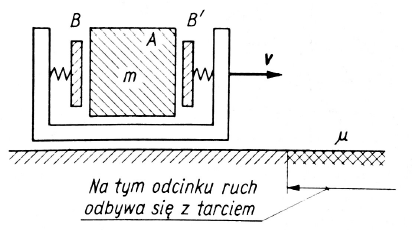
\includegraphics[width=0.4\linewidth]{../rysunki/dynamika/dwa-dynamometry}
\end{figure}

%Kruczek 5_8/51
%Poziom A
